\documentclass{beamer}

\usetheme{Madrid}

\usepackage[utf8]{inputenc}
\usepackage[T1]{fontenc}
\usepackage{amsmath}
\usepackage{amsfonts}
\usepackage{amssymb}
\usepackage{tikz}
\usetikzlibrary{quantikz}
\usepackage{lineno}
\usepackage{multirow}

\title{Quantum Computing and Cryptography}
\author{Damien, Théo, Matthieu}
\institute{}
\date{February 12, 2025}

\begin{document}

\begin{frame}
\maketitle
\end{frame}

\begin{frame}{Outline}
\tableofcontents
\end{frame}

\section{Intro}
\begin{frame}
  \frametitle{Outline}
  \tableofcontents[currentsection]
\end{frame}

\begin{frame}{Introduction}
\begin{linenumbers}
	\begin{itemize}
		\item Cryptography=TODO
		\item TODO: secret
		\item<2->[$\rightarrow$] Science of secret
	\end{itemize}
\end{linenumbers}
\end{frame}

\section{RSA}
\begin{frame}
  \frametitle{Outline}
  \tableofcontents[currentsection]
\end{frame}

\begin{frame}{RSA}
\begin{linenumbers}

\end{linenumbers}
\end{frame}

\section{Quantum computing}
\begin{frame}
  \frametitle{Outline}
  \tableofcontents[currentsection]
\end{frame}

\begin{frame}{Quantum computing}
	\centering
	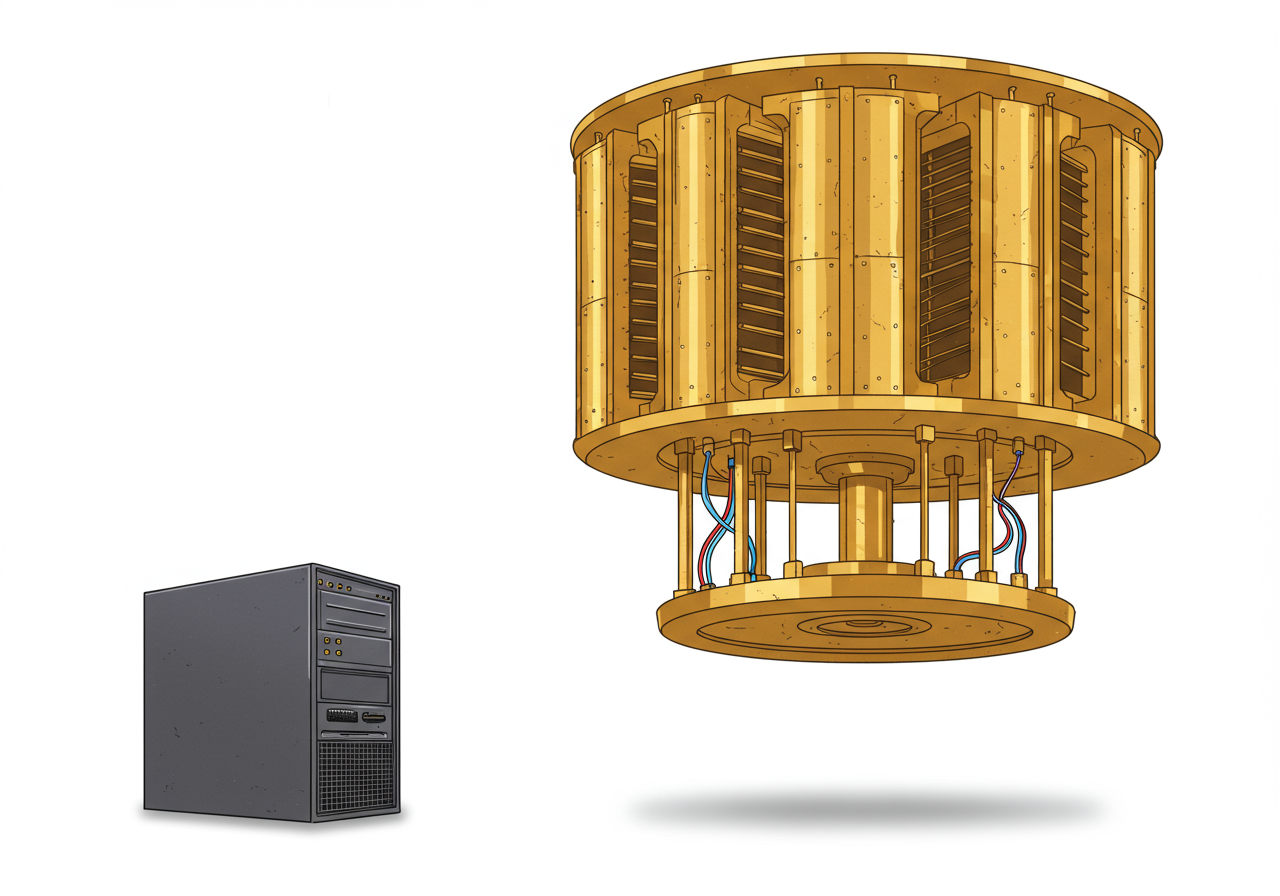
\includegraphics[width=0.8\textwidth]{classical-vs-quantum.png}
\end{frame}

\subsection{Introduction to the quantum world}
\begin{frame}
  \frametitle{Outline}
  \tableofcontents[currentsection,currentsubsection]
\end{frame}

\subsubsection*{Qubits}
\begin{frame}{Qubits}
\begin{linenumbers}
	\begin{block}<+->{Classical bit}
		$b \in \{0, 1\}$
		\begin{itemize}[<+->]
			\item $0$
			\item $1$
		\end{itemize}
	\end{block}

	\begin{block}<+->{Quantum bit}
		$\ket{\psi} \in \mathbb{C}^2$
		\begin{columns}[T,onlytextwidth]
			\column{0.5\textwidth}
				\begin{itemize}[<+->]
					\item $\ket{0} = \begin{bmatrix} 1 \\ 0 \end{bmatrix}$
					\item $\ket{1} = \begin{bmatrix} 0 \\ 1 \end{bmatrix}$
				\end{itemize}
			\column{0.5\textwidth}
				\begin{itemize}[<+->]
					\item $\ket{+} = \frac{1}{\sqrt{2}}\begin{bmatrix} 1 \\ 1 \end{bmatrix}$
					\item $\ket{-} = \frac{1}{\sqrt{2}}\begin{bmatrix} 1 \\ -1 \end{bmatrix}$
				\end{itemize}
		\end{columns}
	\end{block}
\end{linenumbers}
\end{frame}


\subsubsection*{Measurements}
\begin{frame}{Measurements}
	\begin{linenumbers}
		\begin{block}<+->{Why measuring ?}
			We cannot read superposition. When we look at a qubit, it collapses to a classical bit.
		\end{block}
		\begin{block}<+->{What do we get ?}
			We measure $0$ or $1$ with a probability that depends on the state of the qubit.
			\begin{itemize}[<+->]
				\item $\ket{0}$ $\rightarrow 0$ (100\%)
				\item $\ket{1}$ $\rightarrow 1$ (100\%)
				\item $\ket{+}$ $\rightarrow 0$ (50\%), $1$ (50\%)
				\item $\ket{-}$ $\rightarrow 0$ (50\%), $1$ (50\%)
			\end{itemize}
		\end{block}
	\end{linenumbers}
\end{frame}

\subsubsection*{Gates}
\begin{frame}{NOT gate}
\begin{linenumbers}
    \begin{block}<+->{X gate}
			\begin{itemize}
					\item $X\ket{0} \rightarrow \ket{1}$
					\item $X\ket{1} \rightarrow \ket{0}$
			\end{itemize}
		\end{block}
		\begin{block}<+->{Circuit representation}
			\centering
			\begin{quantikz}
				\lstick{$\ket{\psi}$} & \gate{X} & \meter{}
			\end{quantikz}
    \end{block}
\end{linenumbers}
\end{frame}

\begin{frame}{Hadamard gate}
	\begin{block}<+->{H gate}
			\begin{itemize}
					\item $H\ket{0} \rightarrow \ket{+}$
					\item $H\ket{1} \rightarrow \ket{-}$
			\end{itemize}
	\end{block}
	\begin{block}<+->{Circuit representation}
			\centering
			\begin{quantikz}
					\lstick{$\ket{\psi}$} & \gate{H} & \meter{}
			\end{quantikz}
	\end{block}
\end{frame}

\subsection{Quantum algorithms}
\begin{frame}
  \frametitle{Outline}
  \tableofcontents[currentsection,currentsubsection]
\end{frame}

\subsubsection*{Bernstein-Vazirani Problem}
\begin{frame}{Bernstein-Vazirani Problem}
\begin{linenumbers}
  \begin{block}<+->{Problem Definition}
    Given an oracle for a function $f$:
    \[ f : \{0, 1\}^n \rightarrow \{0, 1\} \]
    \[ f(\mathbf{x}) = \mathbf{x} \cdot \mathbf{s} \]
    where $\mathbf{s}$ is a secret bit string. Find $\mathbf{s}$ with the fewest oracle calls.  ($\cdot$ is the bitwise dot product, XOR sum).
  \end{block}
\end{linenumbers}
\end{frame}

\subsubsection*{Classical Algorithm}
\begin{frame}{Classical Algorithm - Example}
\begin{linenumbers}
  \begin{block}<+->{Example (n=2)}
    To find $\mathbf{s} = s_0s_1$:
    \begin{itemize}[<+->]
        \item Query $f(10)$.  Result: $s_0$.
        \item Query $f(01)$.  Result: $s_1$.
    \end{itemize}
    Requires 2 queries.
  \end{block}
\end{linenumbers}
\end{frame}


\begin{frame}{Classical Algorithm - General Case}
	\begin{linenumbers}
		\begin{block}<+->{Complexity: $\mathcal{O}(n)$}
			We need to isolate each bit of $\mathbf{s}$ by querying with inputs that have a single '1'. This requires $n$ queries for an $n$-bit string.
		\end{block}
	\end{linenumbers}
	\end{frame}
	

\subsubsection*{Quantum Algorithm}
\begin{frame}{Quantum Algorithm - Overview}
\begin{linenumbers}
	\begin{block}<+->{Complexity: $\mathcal{O}(1)$}
		The quantum algorithm can find $\mathbf{s}$ with just *one* query.  It uses superposition to query all possible inputs simultaneously.
	\end{block}
\end{linenumbers}
\end{frame}

% \begin{frame}{Algo Quantique - Slide 2}
% \begin{linenumbers}
% 	\begin{quantikz}
% 		\lstick{} & \gate{H} & \gate[2]{U_f} & \gate{H} & \meter{} & \qw \\
% 		\lstick{} & \gate{H} &               & \gate{H} & \meter{} & \qw
% 		\end{quantikz}
% \end{linenumbers}
% \end{frame}

\begin{frame}{Quantum Algorithm - Circuit}
	\begin{linenumbers}
		\begin{block}<+->{Circuit Diagram}
			\centering
			\begin{quantikz}
				\lstick{} & \gate{H} & \gate[2]{U_f} & \gate{H} & \meter{} & \qw \\
				\lstick{} & \gate{H} &               & \gate{H} & \meter{} & \qw
				\end{quantikz}
		\end{block}
			\begin{block}<+->{Explanation}
			\begin{itemize}[<+->]
					\item  $H^{\otimes n}$ : Hadamard gates on all n input qubits (creates superposition).
					\item $U_f$ : The quantum oracle.
					\item Final Hadamards and measurement reveal $\mathbf{s}$.
			\end{itemize}
	\end{block}
	\end{linenumbers}
	\end{frame}

% \subsubsection*{Shor}
% \begin{frame}{Shor}
% \begin{linenumbers}
%     \begin{itemize}[<+->]
%         \item Gain de complexité :
%         $\mathcal O(e^b)$ $\rightarrow$ $\mathcal O(b³)$
%         \item combien de qubit il faut
%         \item combien de cubit on as
%     \end{itemize}
% \end{linenumbers}
% \end{frame}

\subsubsection*{Shor's Algorithm}
\begin{frame}{Shor's Algorithm}
\begin{linenumbers}
  \begin{block}<+->{Complexity Gain}
        Classical factoring is very slow (roughly $\mathcal{O}(e^{\sqrt[3]{n}})$). Shor's algorithm is much faster (polynomial, $\mathcal{O}((\log N)^3)$).
  \end{block}
    \begin{block}<+->{Requirements}
        \begin{itemize}[<+->]
            \item Requires a large number of high-quality (low-error) qubits (roughly $2n$ for an $n$-bit number).
            \item  We currently don't have quantum computers large and stable enough to break practical RSA encryption.
        \end{itemize}
    \end{block}
\end{linenumbers}
\end{frame}

\section{Post-Quantum cryptography}
\begin{frame}
  \frametitle{Outline}
  \tableofcontents[currentsection]
\end{frame}

\subsection{Intro to PQ cryptography}
\begin{frame}
  \frametitle{Outline}
  \tableofcontents[currentsection,currentsubsection]
\end{frame}

\begin{frame}{What is PQ cryptography}
\begin{linenumbers}
	\begin{itemize}
		\item Based on (other) mathematical problems
		\item Considered unsolvable by a quantum computer
	\end{itemize}

	What it is not :
	\begin{itemize}
		\item Cryptography \textbf{using} quantum technologies
	\end{itemize}
\end{linenumbers}
\end{frame}

\begin{frame}{The problems}
	\begin{itemize}
		\item Codes
		\item Hash functions
		\item Multivariates polynomials systems
		\item Isogenies
		\item {\color<2>{red} Lattices}
	\end{itemize}
\end{frame}

\begin{frame}{Why lattices ?}
	\begin{itemize}
		\item Well spread
		\item Good results
			\begin{table}[h!]
			\begin{tabular}{|c|c|}
				\hline
				\multicolumn{2}{|c|}{Encryption/Key encapsulation} \\
				\hline
				Crystals-Kyber & Lattices \\
				\hline
				\multicolumn{2}{|c|}{Signatures} \\
				\hline
				Crystals-Dilithium & Lattices \\
				Falcon & Lattices \\
				Sphincs+ & Hash \\
				\hline
			\end{tabular}
			\end{table}
	\end{itemize}
\end{frame}

\subsection{Lattice cryptography}
\begin{frame}
  \frametitle{Outline}
  \tableofcontents[currentsection,currentsubsection]
\end{frame}

\subsubsection{What is a lattice ?}
\begin{frame}{Some definitions}
	\begin{itemize}
		\item A discret subgroup of $RR^n$
	\end{itemize}

	Like vector spaces, we have :
	\begin{itemize}
		\item Vectors and matrices
		\item Linear combination
	\end{itemize}
\end{frame}

\begin{frame}{Example}
	\begin{columns}[t]
	\begin {column}{0.5\textwidth}
		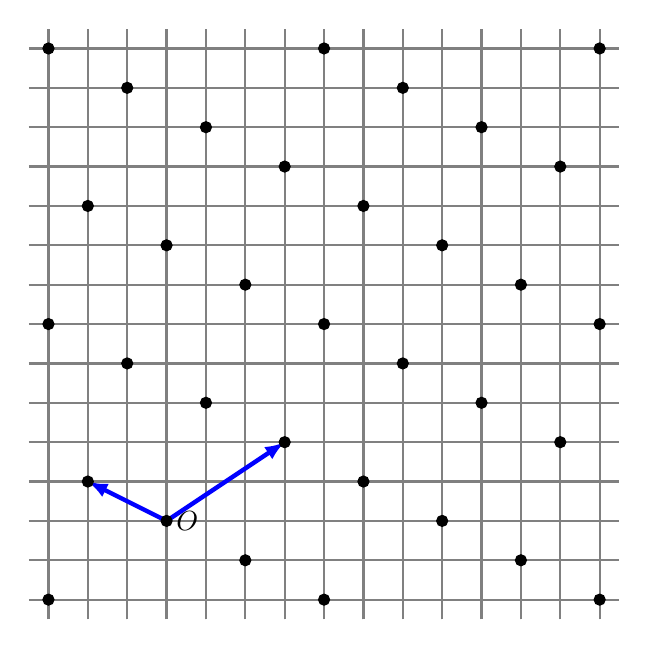
\begin{tikzpicture}
		\foreach \i in {1, ..., 8, 1.5, ..., 7.5} {
			\draw [gray, thick] (\i, 0.75) -- (\i, 8.25);
		}
		\foreach \i in {1, ..., 8, 1.5, ..., 7.5} {
			\draw [gray, thick] (0.75, \i) -- (8.25, \i);
		}

		%%% Basis
		\draw[ultra thick, blue, arrows={-{Latex[length=2.5mm]}}] (2.5, 2) -- (4, 3);
		\draw[ultra thick, blue, arrows={-{Latex[length=2.5mm]}}] (2.5, 2) -- (1.5, 2.5);

		%%% The lattice's points
		\filldraw[black] (8, 1) circle (2pt);

		\filldraw[black] (7, 1.5) circle (2pt);

		\filldraw[black] (4.5, 1) circle (2pt);
		\filldraw[black] (6, 2) circle (2pt); % end
		\filldraw[black] (7.5, 3) circle (2pt);

		\filldraw[black] (3.5, 1.5) circle (2pt);
		\filldraw[black] (5, 2.5) circle (2pt);
		\filldraw[black] (6.5, 3.5) circle (2pt); % end
		\filldraw[black] (8, 4.5) circle (2pt);

		\filldraw[black] (1, 1) circle (2pt); % beg
		\filldraw[black] (2.5, 2) circle (2pt) node[anchor=west]{$O$};
		\filldraw[black] (4, 3) circle (2pt);
		\filldraw[black] (5.5, 4) circle (2pt);
		\filldraw[black] (7, 5) circle (2pt); % end

		\filldraw[black] (1.5, 2.5) circle (2pt); % beg
		\filldraw[black] (3, 3.5) circle (2pt);
		\filldraw[black] (4.5, 4.5) circle (2pt);
		\filldraw[black] (6, 5.5) circle (2pt);
		\filldraw[black] (7.5, 6.5) circle (2pt); % end

		\filldraw[black] (2, 4) circle (2pt); % beg
		\filldraw[black] (3.5, 5) circle (2pt);
		\filldraw[black] (5, 6) circle (2pt);
		\filldraw[black] (6.5, 7) circle (2pt);
		\filldraw[black] (8, 8) circle (2pt); % end

		\filldraw[black] (1, 4.5) circle (2pt);
		\filldraw[black] (2.5, 5.5) circle (2pt); % beg
		\filldraw[black] (4, 6.5) circle (2pt);
		\filldraw[black] (5.5, 7.5) circle (2pt);

		\filldraw[black] (1.5, 6) circle (2pt);
		\filldraw[black] (3, 7) circle (2pt);  % beg
		\filldraw[black] (4.5, 8) circle (2pt);

		\filldraw[black] (2, 7.5) circle (2pt);

		\filldraw[black] (1, 8) circle(2pt);
		\end{tikzpicture}
	\end{column}
	\begin{column}{0.45\textwidth}
		FIXME : Basis:

		\[\left\{\left(\begin{matrix}3\\2\end{matrix}\right), \left(\begin{matrix}-2\\1\end{matrix}\right)\right\}\]
	\end{column}
	\end{columns}
\end{frame}

\begin{frame}{Learning with error problem}
	TODO
\end{frame}

\begin{frame}{(Fully) homomorphic encryption}
	\begin{itemize}
		\item Based on lattices (variant of LWE problem)
		\item<2-> We can evaluate a circuit (operations) on encrypted data
		\item<2-> Two operations : $+$ and $\cdot$, forms a ring
		\item<3-> We can evaluate (or compile) a function $f : P \times P \rightarrow P$ on encrypted data $C_1$ and $C_2$ :
			\[eval(f, C_1, C_2) = Enc(f(Dec(C_1), Dec(C_2)))\]
		\item<4-> Used to manipulate private data (e.g. Medical data, data science)
	\end{itemize}
\end{frame}

\subsection{Limits of PQ cryptography}
\begin{frame}
  \frametitle{Outline}
  \tableofcontents[currentsection,currentsubsection]
\end{frame}
\begin{frame}{Sizes of the keys and data}
	\begin{tabular}{|c|c|}
		\hline
		TODO & \\
		\hline
	\end{tabular}
\end{frame}

\begin{frame}{Not necessarly robust to classical computer}
	\begin{itemize}
		\item Example : Supersingular isogenies Diffie-Hellman key exchange
	\end{itemize}
\end{frame}

\section{Conclusion}
\begin{frame}
  \frametitle{Outline}
  \tableofcontents[currentsection]
\end{frame}
\begin{frame}{Conclusion}
\begin{linenumbers}
    % Content from brouillon.md - To be filled
\end{linenumbers}
\end{frame}

\end{document}
